% Created 2014-11-17 Mon 13:42
\documentclass[presentation, bigger]{beamer}
\usepackage[utf8]{inputenc}
\usepackage[T1]{fontenc}
\usepackage{fixltx2e}
\usepackage{graphicx}
\usepackage{longtable}
\usepackage{float}
\usepackage{wrapfig}
\usepackage{rotating}
\usepackage[normalem]{ulem}
\usepackage{amsmath}
\usepackage{textcomp}
\usepackage{marvosym}
\usepackage{wasysym}
\usepackage{amssymb}
\usepackage{hyperref}
\tolerance=1000
\usetheme{kuleuven}
\useinnertheme{rectangles}
\graphicspath{{graphics/}}
\usepackage[dutch, english]{babel}
\usepackage{graphicx}
\usepackage{tikz}
\usetikzlibrary{intersections}
\usetheme{default}
\author{Ward Schodts, Xavier Goás Aguililla}
\date{maandag 10 november 2014}
\title{Internet of Things code deployment metrics: probleemstelling}


\let\otp\titlepage
\renewcommand{\titlepage}{\otp\addtocounter{framenumber}{-1}}

\setbeamertemplate{frametitle}
{
  \vskip 2mm
  {\insertframetitle} \hfill {\normalsize \textbf{\insertframenumber/\inserttotalframenumber}} %section number, frame title and slide number
}

\hypersetup{
  pdfkeywords={},
  pdfsubject={},
  pdfcreator={Emacs 24.4.1 (Org mode 8.2.10)}}
\begin{document}

\begin{frame}[plain]
 \titlepage
\end{frame}

\begin{frame}[label=sec-1]{Slide 1}
\begin{itemize}[<+->]
\item Observatie\\

  \begin{itemize}
  \item in WSN's weinig gebruik van CPU \& flash
  \end{itemize}
\note{
In WSNs wordt weinig gebruik gemaakt van de ingebedde rekenkracht en
opslagcapaciteit van de sensor nodes.
}

\item Vraagstelling\\
  \begin{itemize}
  \item andere, misschien betere, aanpak mogelijk?
  \end{itemize}

\note{
Zou het mogelijk zijn om een andere aanpak te gebruiken, d.i. meer
berekeningen uit te voeren en meer data op te slaan op de sensor nodes
zelf, zonder verlies van performantie of energie-efficiëntie?
}
\item Waarom\\
\note{
  \begin{itemize}
  \item gereduceerd energieverbruik
  \item efficiënter netwerk
  \end{itemize}
Als dit mogelijk was dan zouden we minder gebruik moeten maken van de
RF-antennes, die veel energie verbruiken. Eventueel kan dit zelfs ook
betere performantie opleveren, omdat er dan minder data over het
netwerk zou moeten overgedragen worden.
}
\end{itemize}
\end{frame}
\begin{frame}[label=sec-2]{Slide 2}
\begin{itemize}[<+->]
\item Hypothese\\
  \begin{itemize}
  \item in sommige scenario's beter om CPU \& flash te gebruiken
  \end{itemize}
\note{
Wij denken dat in bepaalde scenario's het beter is om bewerkingen op
de sensor nodes uit te voeren voor een efficiënter energiegebruik en
misschien zelfs betere performantie.
}
\item Bewijs\\
  \begin{itemize}
  \item metingen voor zelfde fysieke setup met energie- en performantiewinst
  \end{itemize}
\note{
Metingen die aantonen dat voor een gelijkaardige fysieke setup een
andere verdeling van de werklast binnen het WSN voordelen oplevert qua
energieverbruik en/of performantie vis-à-vis een klassiekere
werkverdeling.
}
\item Vereisten\\
  \begin{itemize}
  \item simulatietool op basis van type node en code deployment
  \end{itemize}
\note{
Het ontwikkelen van een tool die toelaat om de potentiële
energie-efficiëntie en performantie van een WSN te meten op basis
van welke types code (bv. adhv. vooraf gebenchmarkte API calls) waar
worden uitgevoerd.
}
\end{itemize}
\end{frame}
\begin{frame}[label=sec-3]{Pyramide}
\begin{minipage}{.5\textwidth}
\centering
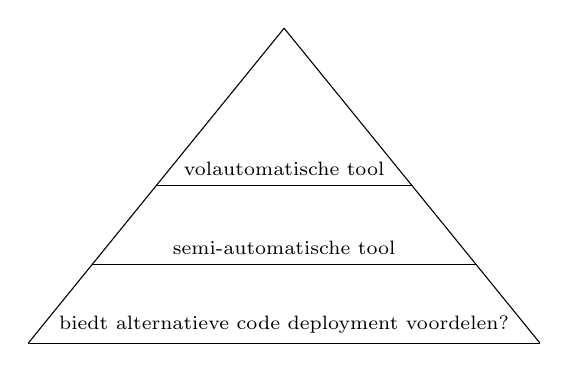
\begin{tikzpicture}
\coordinate (A) at (-3.25,0) {};
\coordinate (B) at ( 3.25,0) {};
\coordinate (C) at (0,4) {};
\draw[name path=AC] (A) -- (C);
\draw[name path=BC] (B) -- (C);
\foreach \y/\A in {0/\scriptsize{biedt alternatieve code deployment voordelen?},1/\scriptsize{semi-automatische tool},2/\scriptsize{volautomatische tool}} {
    \path[name path=horiz] (A|-0,\y) -- (B|-0,\y);
    \draw[name intersections={of=AC and horiz,by=P},
          name intersections={of=BC and horiz,by=Q}] (P) -- (Q)
        node[midway,above] {\A};
}
\end{tikzpicture}
\end{minipage}%
\begin{minipage}{.5\textwidth}
\centering
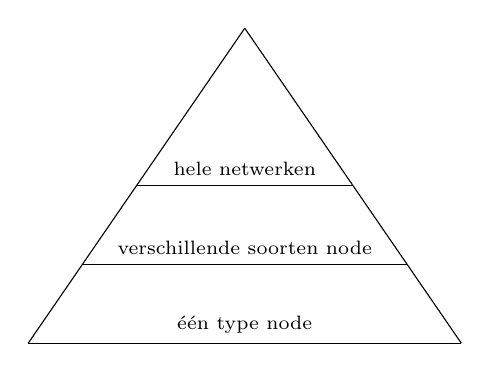
\begin{tikzpicture}
\coordinate (A) at (-2.75,0) {};
\coordinate (B) at ( 2.75,0) {};
\coordinate (C) at (0,4) {};
\draw[name path=AC] (A) -- (C);
\draw[name path=BC] (B) -- (C);
\foreach \y/\A in {0/\scriptsize{\'e\'en type node},1/\scriptsize{verschillende soorten node},2/\scriptsize{hele netwerken}} {
    \path[name path=horiz] (A|-0,\y) -- (B|-0,\y);
    \draw[name intersections={of=AC and horiz,by=P},
          name intersections={of=BC and horiz,by=Q}] (P) -- (Q)
        node[midway,above] {\A};
}
\end{tikzpicture}
\end{minipage}
\end{frame}
% Emacs 24.4.1 (Org mode 8.2.10)
\end{document}